\chapter{State of the art}
\label{state_of_art}

\section{Introduction}
The aim of this chapter is to present the main goal that document classification should achieve. Each of required steps with a variety of available methods is shown and briefly described followed by real use cases. The chapter starts with introducing the concept of data mining in large data sets. In next section of this chapter methods of extraction best features that represent sample and allow to distinguish documents with each other will be discussed. In next two sections of this chapter concepts of data clusterization and classification will be introduced along with known algorithms. Fourth section deals with problems associated with documents classification performance, describing methods for distributing data across cluster of nodes and performing scalable tasks. Finally, taking into consideration all aspects that were raised in previous sections, the general concept of text document classification with associated problems will be explained.

\section{Background}
The manual pattern identification has been known since early 1700s, when Bayes' theorem was discovered \cite{bayesian-history}. However the increasing power of computer technology has lead to fast increment of data collection. Over the past decades, text documents became more and more accessible, because of digitalization of information, introducing strong need for efficient storage and fast information lookup \cite{digitalization}. Both of those needs have caused two questions to grow in importance - how to classify given document with certain confidence of accuracy in relevance to the set of other documents, and how to perform such task in acceptable time frame.

As digital document archives has grown in number and complexity, manual data analysis has been augmented with automatic algorithms of data processing aided by such discoveries as neural networks or decision trees. Application of these methods motivated by uncovering hidden patterns in dataset is known as data mining, an interdisciplinary subfield of computer science \cite{data-mining}. This process is an analysis step of the Knowledge Discovery in Databases, which aims at extracting patterns from dataset and transform them into structures that could be further used \cite{data-mining-kdd}. 

The process of Knowledge Discovery in Databases can be divided into following steps:

\begin{enumerate}
	\item \textbf{Pre-processing} - it is necessary to assemble the target dataset before applying data mining algorithms. Preparing the target dataset is not an easy task because it must be large enough to contain patterns while remaining concise enough to be processed in acceptable time period. In this step the target set is often cleaned to remove noise, missing data or data that does not provide valuable information.
	\item \textbf{Data mining} - the actual process of pattern extraction, which involves:
		\begin{itemize}
			\item \textbf{anomaly detection} - finding unusual data samples that require further investigation
			\item \textbf{dependency modeling} - association rule learning to find relations between variables, for example \textit{Apriori algorithm, decision tree}
			\item \textbf{clustering} - known as \textit{unsupervised learning} - finding groups of data without any supervision \cite{fe_signal_processing}, , for example \textit{K-means algorithm, K-nearest neighbour algorithm, Hierarchical algorithm}
			\item \textbf{classification} - known as \textit{supervised training} - training classifier with the labeled examples to create a set of rules or model that can search for feachures captured from a new sample and label it \cite{fe_signal_processing}, , for example \textit{Bayesian classifier, Naive Bayes}
			\item \textbf{regression} - finding a function which can model the dataset with the least error
			\item \textbf{summarization} - representation of the data
		\end{itemize}
	\item \textbf{Results validation} - the final step of Knowledge Discovery process is to verify whether discovered patterns can be applied to a wider dataset. It may turned out to be impossible to use some of the patters and reproduce results on a new sample. The process of using the model that is excessively complex and includes too many parameters in statistics and machine learning is known as over-fitting. A model that has been overfit may have poor predictive performance, as it  exaggerates even small fluctuations of information.  The accuracy of the model can then be measured from how many of new samples are correctly classify based on patterns learned from the training set. The binary classificator can also be evaluated by some statistical methods, for example the receiver operating characteristic, ROC.
	
	
	
\end{enumerate} 




\section{Knowledge Discovery in Databases}
\subsection{Pre-processing}
When designing a classifier for text documents, the feature extraction step is one of the most crucial to the final outcome. It should be build regarding the context that it is going to be used in, or it might render final solution to be inaccurate.
One must remember that the choice of right feature can dramatically affect the achieved results and outcome. Feature extraction is most commonly used in signal and image processing \cite{fe_signal_processing}. In this case the features are purely mathematical concepts, like wavelet coefficients or geometric measures, which include perimeter, compactness, major and minor axes, eccentricity or Fourier Descriptors. In the presented case the problem is not so trivial. Many features might be unidentified or unnamed. However, it is very important to extract them, as they might have potential of improving classification or clustering significantly.
In this step of Knowledge Discovery in Databases process, the target set is prepared and then, data mining algorithms are applied to it in order to find characteristic patterns.
Some ways of cleaning and generalizing existing information are described below.
	\subsubsection{Bag of words}
	The process of lemmatization and stemming are the normalization techniques which allows to create a connection between base word and word modifications. This normalization is essential in various
	natural language processing (NLP) systems, for example text classification and
	information extraction, as it brings out actual grammatical or semantic
	meanings which are not accessible by the software \cite{lemma}.

\begin{enumerate}

\item	\textbf{Stemming}
	
	Stemming is a process of getting word stem from its inflected and derived forms. The main algorithm criteria is the fact that the stem has to be identical to the morphological root. There are several types of stemming algorithms. Each of them differs in respect to accuracy and achieved performance.
	
	\begin{enumerate}
		\item \textbf{Lookup algorithms} - In this approach each of the inflected form together with related stem is collected in the structured form  \cite{lookup-stem}, a lookup table (def. \ref{lookup-table}). If a proper table is prepared, the algorithm is very efficient and fast. However the process of creating the table may be quite long and the table itself can be very large. Moreover for every new word it has to be updated. 
		
		 \begin{definition}[Lookup table]
		 	\label{lookup-table}
		 	Lookup table - an array that replaces runtime computation with an array indexing operation
		 	
		 \end{definition}
	
		
		\item \textbf{Suffix-stripping algorithms} - The main goal of suffix stripping is to reduce the size and complexity of the data. As mentioned in \cite{suffix-stripping} generally a document is represented by a vector of words. Suffix-stripping algorithm takes advantage of the fact that usually words with the same stem will have a similar meaning, for example: \textit{connect, connected, connection}. Removal of these suffixes may lead to improving performance of document classification and clustering because of conflating groups of terms into a single term. 
		
		There are several strategies and approaches to suffix stripping, for example using stem dictionary or suffix list. However defining a list of suffixes with various rules is correspondingly difficult. In some cases a combination of letters may really be a suffix, while in others it may be in fact a part of the stem and its removal is unhelpful, because the meaning of the word will be altered. One example that illustrates this problem is ER ending. Conflating words SAND and SANDER is correct, but for WAND and WANDER it is an error. 
		That it way this problem is not so trivial and system of this kind can easily become very complex because of a need to specify many additional rules \cite{suffix-stripping}.
 

		
	\end{enumerate}
	
\item	 \textbf{Lemmatisation}
	 
	 The lemmatisation algorithm reduces inflectional forms of a word to a base/root form (or dictionary form known as \textit{lemma}) by using vocabulary and morphological analysis of words. This process is similar, but not identical to stemming \cite{lemma}. 
	 At first the part of speech of a word is determined, and then different normalization rules for each part of speech are applied. The algorithm is limited by the possibility to obtain the correct lexical category.
	 
\item	\textbf{Stochastic algorithms} 
	
	In this method, a probabilistic model is developed and used to identify the base form of a word. This model usually consist of a wide range of complex linguistic rules. Some lemmatisation algorithms may also be stochastic, because a word may belong to more than one parts of speech. In this case a probability is assigned to each possible part. 
	
\item	\textbf{Term Frequency, (Inverse) Document Frequency}

This is a numerical statistic which specifies how important a word is to a document in a text corpus (def. \ref{corpus}). The tf-idf ratio increases proportionally to the number of occurrences of a word in a document and as a result may be used as a weighting factor \cite{term-frequency}.

	 \begin{definition}[Text corpus]
	 	\label{corpus}
	 	Text corpus - in linguistics a large set of documents 
	 	
	 \end{definition}
\end{enumerate}
	
	
\subsection{Data mining - Dependency modeling}
Dependency modeling focuses on finding association rules using various measures of interestingness \cite{association-rules}. Association rule learning is a popular method for discovering interesting relations between variables. Generally the association rule is a rule that determines a data set that could be found in the database if the other data set exists in this database. In order to select interesting rules, some constraints have to be defined:
 \begin{definition}[Support]
 	\label{support}
 	Support value of X is the proportion of transactions that contain a certain data set \textbf{X}
 	
 \end{definition}
  \begin{definition}[Confidence]
  	\label{confidence}
  	Confidence value of an association rule \[\left \{ X \right \} \Rightarrow \left \{ Y\right \}\] is the proportion of transactions that contain a certain data set \textbf{X} and also the other data set \textbf{Y}
  	
  \end{definition}

\subsubsection{Apriori algorithm}
The Apriori algorithm helps to find which variables can depend on others. 
For example, the rule can look as follows \[\left \{ bread, cheese \right \} \Rightarrow \left \{ butter \right \}\] 
It means that if someone buys bread and cheese, he buys also butter. Such information can
be used as the basis for decisions about marketing activities.
The steps of the Apriori algorithm will be described using following example:
\begin{enumerate}
	\item Consider following transactions gathered in a database presented in the table \ref{apriori-1}
	\begin{table}[H]
		\centering
		\caption{Apriori algorithm - example of transactions}
		\label{apriori-1}
		\begin{tabular}{|c|c|l}
			\cline{1-2}
			Transaction & Items       &  \\ \cline{1-2}
			1           & \{1,2,3,4\} &  \\ \cline{1-2}
			2           & \{1,2\}     &  \\ \cline{1-2}
			3           & \{2,3,4\}   &  \\ \cline{1-2}
			4           & \{1,2,3\}   &  \\ \cline{1-2}
			5           & \{2,3\}     &  \\ \cline{1-2}
		\end{tabular}
	\end{table}
	\item  The Apriori algorithm will be used to determine the frequent item sets of this database. We will assume that an item set is frequent if it appears in at least N transactions. This value (N) is the support threshold.
	\item At first we will count the support of each item separately.
	\begin{table}[H]
		\centering
		\caption{Apriori algorithm - support of each item}
		\label{apriori-2}
		\begin{tabular}{|c|c|l}
			\cline{1-2}
			Item  & Support      &  \\ \cline{1-2}
			\{1\} & 3			 &  \\ \cline{1-2}
			\{2\} & 5            &  \\ \cline{1-2}
			\{3\} & 4            &  \\ \cline{1-2}
			\{4\} & 2            &  \\ \cline{1-2}
		\end{tabular}
	\end{table}
	\item Let the support threshold equals 3 (N=3). As a result all of the items, except item \{4\} are frequent. 
	\item In the next step we generate a list of pairs of frequent items.
	\begin{table}[H]
		\centering
		\caption{Apriori algorithm - support of each pair}
		\label{apriori-3}
		\begin{tabular}{|c|c|l}
			\cline{1-2}
			Item    & Support &  \\ \cline{1-2}
			\{1,2\} & 3       &  \\ \cline{1-2}
			\{1,3\} & 5       &  \\ \cline{1-2}
			\{2,3\} & 4       &  \\ \cline{1-2}
		\end{tabular}
	\end{table}
	\item All of the pairs meet or exceed the minimum support, so they are frequent. Now we can count support of triples. 
	\begin{table}[H]
		\centering
		\caption{Apriori algorithm - support of each triple}
		\label{apriori-4}
		\begin{tabular}{|c|c|l}
			\cline{1-2}
			Item      & Support &  \\ \cline{1-2}
			\{1,2,3\} & 2       &  \\ \cline{1-2}
		\end{tabular}
	\end{table}
	\item Taking into consideration a result collected in the table \ref{apriori-4}, there are no frequent triples in the considered example.
\end{enumerate}
\subsubsection{FP-growth algorithm}
The algorithm for finding frequent patterns is quite simple and includes two passes over the dataset \cite{fp-growth}.
\begin{itemize}
	\item Pass 1
	\begin{enumerate}
		\item support of each item is first counted and stored to 'header table' 
		\item infrequent items are discarded
		\item the FP-tree structure is created by inserting instances into it, items in each instance are sorted by descending order of their frequency
	\end{enumerate}
	\item Pass 2
	\begin{enumerate}
		\item read transactions and map them to a path in the tree
	\end{enumerate}
\end{itemize}
The construction of the FP-tree will be described using following example.
Consider the same database ref{fp-alg} as presented in the Apriori algorithm example.
\begin{table}[H]
	\centering
	\caption{FP-growth algorithm - example of transactions}
	\label{apriori-1}
	\begin{tabular}{|c|c|l}
		\cline{1-2}
		Transaction & Items       &  \\ \cline{1-2}
		1           & \{1,2,3,4\} &  \\ \cline{1-2}
		2           & \{1,2\}     &  \\ \cline{1-2}
		3           & \{2,3,4\}   &  \\ \cline{1-2}
		4           & \{1,2,3\}   &  \\ \cline{1-2}
		5           & \{2,3\}     &  \\ \cline{1-2}
	\end{tabular}
\end{table}
\begin{enumerate}
	\item After reading first transaction 
	\begin{figure}[H]
		\begin{center}
			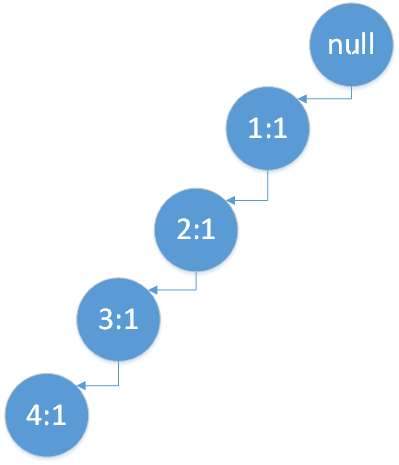
\includegraphics[width=0.4\linewidth]{images/fp1.png}
			\caption{FP-growth example, after reading first transaction}
			\label{fp_1}
		\end{center}
	\end{figure}
	\item After reading second transaction 
		\begin{figure}[H]
			\begin{center}
				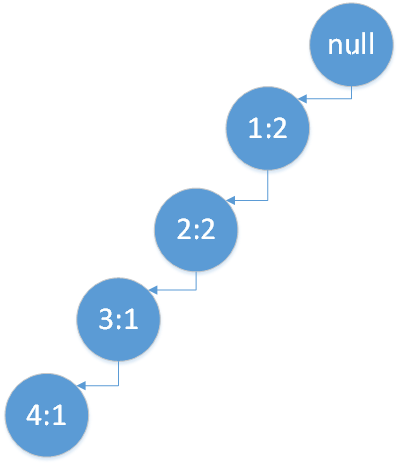
\includegraphics[width=0.4\linewidth]{images/fp2.png}
				\caption{FP-growth example, after reading second transaction}
				\label{fp_2}
			\end{center}
		\end{figure}
			\item After reading third transaction 
			\begin{figure}[H]
				\begin{center}
					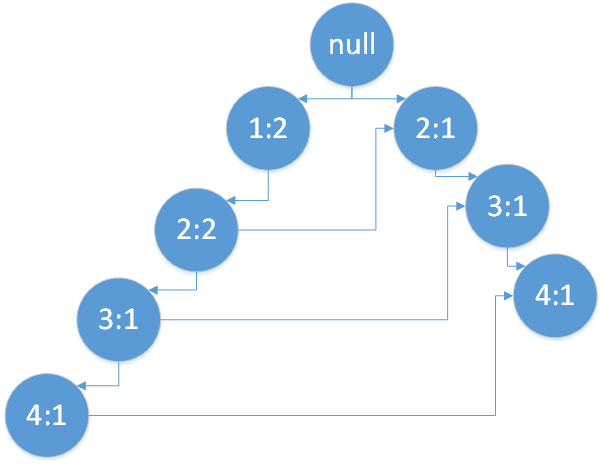
\includegraphics[width=0.4\linewidth]{images/fp3.png}
					\caption{FP-growth example, after reading third transaction}
					\label{fp_3}
				\end{center}
			\end{figure}
				\item After reading fourth transaction 
				\begin{figure}[H]
					\begin{center}
						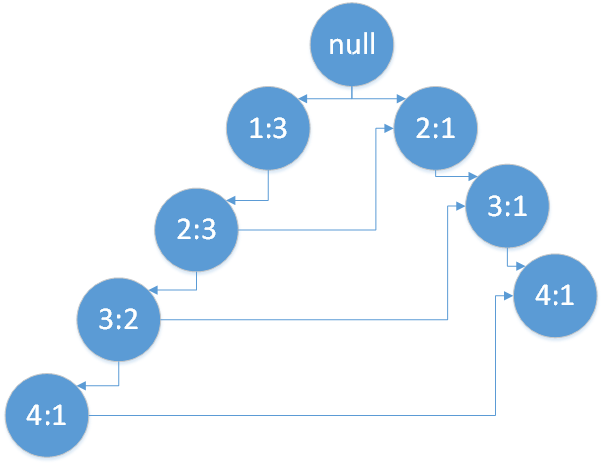
\includegraphics[width=0.4\linewidth]{images/fp4.png}
						\caption{FP-growth example, after reading fourth transaction}
						\label{fp_4}
					\end{center}
				\end{figure}
					\item After reading fifth transaction
					\begin{figure}[H]
						\begin{center}
							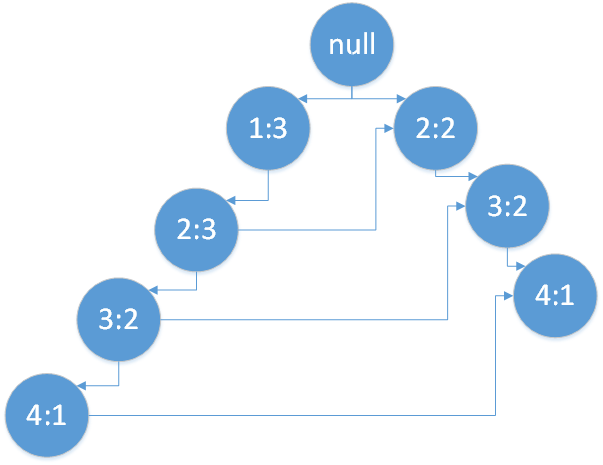
\includegraphics[width=0.4\linewidth]{images/fp5.png}
							\caption{FP-growth example, after reading fifth transaction}
							\label{fp_5}
						\end{center}
					\end{figure}
	
\end{enumerate}


\subsection{Data mining - Documents clusterization}
	\subsubsection{K-means algorithm}
	K-means is one of the most frequently used methods in data clustering. K-means and its derivatives have linear time complexity in relevance to the number of documents \cite{k_means} This algorithm assumes that samples are divided into \textit{K} groups. Its goal is to find the most optimal clusters based on this assumption. Each of clusters has its center and each pattern will be matched to cluster with center closest to matching the pattern. In algorithm, best centers are found in an iterative process.
	
	K-means can be described using following steps and visual example:
	\begin{enumerate}
	
	\item Initialize \textit{k} centers randomly, as presented in Fig. \ref{kmeans_s1}
	\begin{figure}[H]
	\begin{center}
	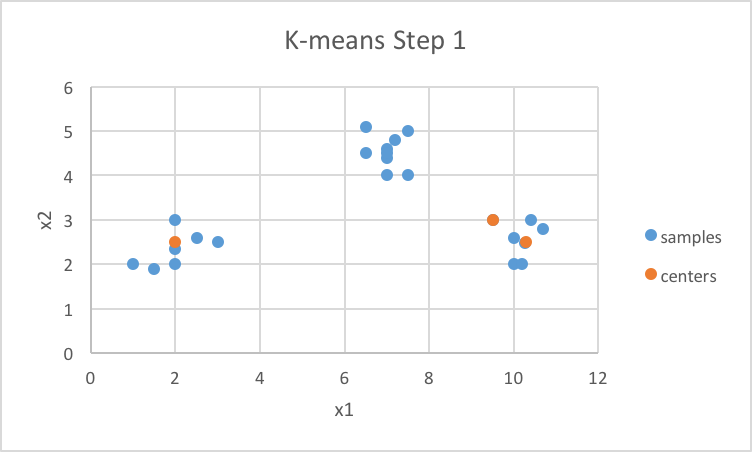
\includegraphics[width=0.8\linewidth]{images/kmeans1.png}
	\caption{K-means algorithm, step 1.}
	\label{kmeans_s1}
	\end{center}
	\end{figure}
	
	\item Find distances between each of centers and each of samples, as presented in Fig. \ref{kmeans_s2}
	\begin{figure}[H]
	\begin{center}
	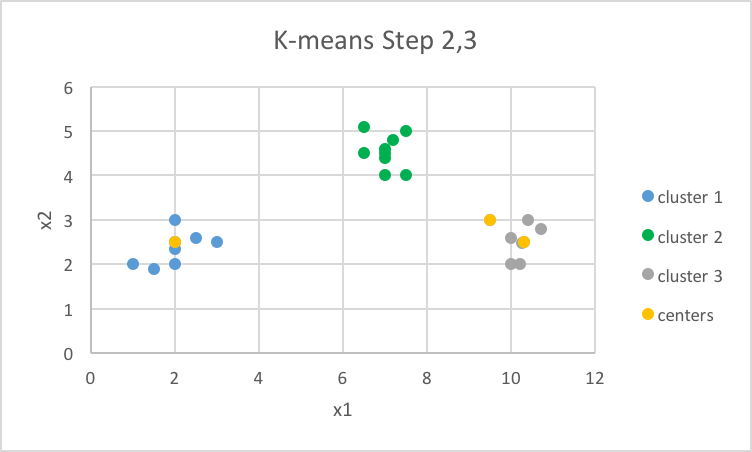
\includegraphics[width=0.8\linewidth]{images/kmeans2.png}
	\caption{K-means algorithm, step 2.}
	\label{kmeans_s2}
	\end{center}
	\end{figure}
	
	\item Assign samples to clusters, for whose calculated distance between sample and cluster's center is minimal, as presented in Fig. \ref{kmeans_s4}
	
	\item Find new cluster centers. New cluster centers are the samples that are positioned closest to the average of all samples in its cluster, , as presented in Fig. \ref{kmeans_s4}
	\begin{figure}[H]
	\begin{center}
	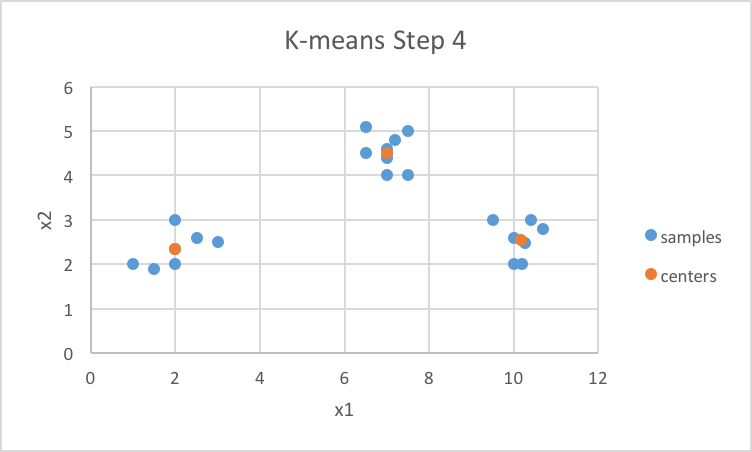
\includegraphics[width=0.8\linewidth]{images/kmeans4.png}
	\caption{K-means algorithm, step 3 \& 4.}
	\label{kmeans_s4}
	\end{center}
	\end{figure}
	
	\item If during previous iteration none of the samples did not change it's cluster, go to next step. Otherwise go back to step 3.
	
	\item Finish. Calculated clusters are the outputs of the algorithm, as presented in Fig. \ref{kmeans_s5}
	\begin{figure}[H]
	\begin{center}
	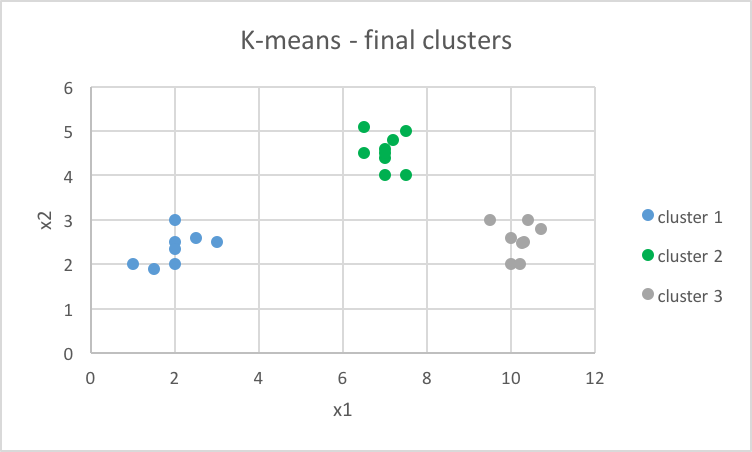
\includegraphics[width=0.8\linewidth]{images/kmeans5.png}
	\caption{K-means algorithm, step 5.}
	\label{kmeans_s5}
	\end{center}
	\end{figure}
	
	\end{enumerate}
	
	\subsubsection{K-Nearest Neighbors algorithm}
	This section focuses on important classification algorithm called K-Nearest Neighbors (kNN). It is simple and efficient to use, as it does not require any labeling for data processing \cite{knn}. KNN is an non parametric lazy learning algorithm, because it doesn't make any assumptions on distribution of information and it doesn't contain any training phase or this phase is very minimal \cite{knn2}.  
	
	In KNN algorithm some assumptions are made:
	\begin{enumerate}
		\item Each training dataset consists of vectors labeled by a class differentiator. 
		\item Data is in feature/metric space, so it is a scalar or multidimensional vector. This assumption is necessary to be able to use a notion of distance \cite{knn2}.
		\item It is necessary to specify a kn number which determines number of neighbors that have influence on classification. 
	\end{enumerate}
	
	The algorithm of labeling a sample using kNN algorithm involves following steps:
	\begin{itemize}
		\item \textbf{Case 1, k=1}

	\begin{enumerate}
		\item Let \textbf{A} be a point, which we want to label.
		\item Find a point \textbf{B}, that is closest to \textbf{A} taking into account the geometrical distance.
		\item Assign label of \textbf{B} to \textbf{A}
		
	\end{enumerate}
	
		\item \textbf{Case 2, k=k}
		\begin{enumerate}
			\item We want to find \textit{k} Nearest Neighbors and perform the majority voting.
			\item Let assume that we have \textit{n} instances of class 1 \textbf{C1} and \textit{n+1} instances of class 2 \textbf{C2}, such as \textit{k=2n+1}
			\item We want to label \textbf{A} sample.
			\item The sample \textbf{A} will be labeled as \textbf{C2}, as it forms majority.
		\end{enumerate}
			\item \textbf{Case 3, weightened kNN} - in this case each point has a weight which is  calculated using the distance to the sample, instead of giving all points weight equals 1. 
		\end{itemize}
		
		Obviously this algorithm may result an error. However this statement holds only when a dataset is not big and the error turns out to be quite small, less than twice the Bayes error rate as described in \cite{duda-hart-classification}. One of the authors statements is to obtain a tight error bound to the Nearest Neighbor Rule:
		\[P*\leqslant P\leqslant P*(2-\frac{c}{c-1}P*)\]
		where:
		\begin{itemize}
			\item \textit{P*} - Bayes error rate
			\item \textit{c} - number of classes
			\item \textit{P} - Nearest Neighbor error rate
		\end{itemize}
	
	
	
	TODO https://www.youtube.com/watch?v=UqYde-LULfs figures
	\begin{enumerate}
	\item Given N training vectors, kNN	algorithm identifies the \textit{k} nearest neighbors of 'c', regardless of labels
	\end{enumerate}
	
	\subsubsection{Hierarchical algorithm}
	Hierarchical clustering is a method which aims to build a hierarchy of clusters. It is often presented as the one that offers better quality, but its use is limited due to quadratic time complexity \cite{k_means}. Hierarchical clustering goal is to produce a tree with single all-inclusive cluster as the root, that than divides into smaller, nested partitions with a single clusters at the bottom. Each of mid-points can be described as a combination of two clusters from lower level or as a part that was produced from splitting higher level. The output of such method can be visualized as a tree that is called dendogram (see Fig. \ref{hierarchical_dendogram}). This clustering offers two approaches, that share mentioned principles:
	
	\begin{itemize}
	\item \textbf{Divisive} (top down) - start with single all-inclusive cluster. At each step divide it into two smaller clusters. With each step it is required to make a decision on which cluster to split and how to perform it.
	\item \textbf{Agglomerative} (bottom up) - start from single clusters, at each step finding the most similar or closest pair, merging it together to form upper intermediate level. Requires definition of similarity or distances of clusters.
	\end{itemize}
	
	\begin{figure}[H]
	\begin{center}
	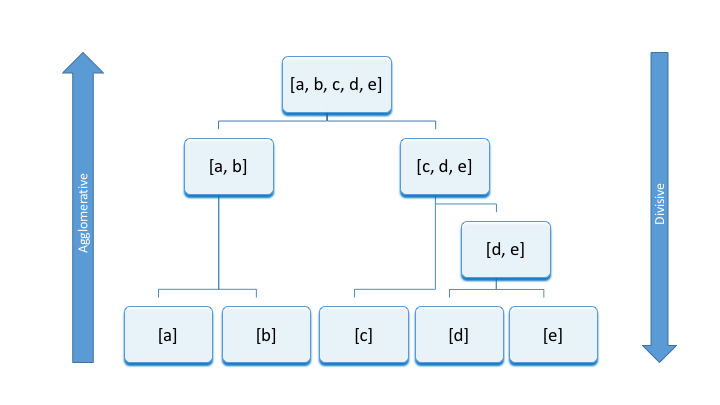
\includegraphics[width=1.0\linewidth]{images/hierarchical.png}
	\caption{Hierarchical algorithm, dendogram example for divisive and agglomerative approach}
	\label{hierarchical_dendogram}
	\end{center}
	\end{figure}

\subsection{Data mining - Documents classification}
	\subsubsection{Support Vector Machine model}
	\subsubsection{Naive Bayes}
	Naive Bayes is a fast statistical classifier which is frequently used in spam detection systems.
	\subsubsection{Maximum Entropy}
	\subsubsection{Winnow}
	\subsubsection{Neural Network}
	\textbf{Perceptrons}
	
\subsection{Results validation}
\subsubsection{Evaluation of binary classifiers}
 The accuracy of the model can be evaluated by some statistical methods.
  The receiver operating characteristic is a graphical plot which presents the true positive rate \textit{TPR} (def. \ref{TPR}) against the false positive rate \textit{FPR} (def. \ref{FPR}).
  
  \begin{definition}[TPR]
  	\label{TPR}
  	TPR - True positive rate, known as sensitivity in signal detection and biomedical engineering and recall in machine learning. It is a rate that measures the proportion of properly classified positive samples:
  	\[TPR=\frac{TP}{TP+FN}\]
  	where:
\begin{enumerate}
  		\item TP - True Positive, correctly identified
  		\item FN - False Negative, incorrectly rejected
\end{enumerate}
  \end{definition}
  \begin{definition}[FPR]
  	\label{FPR}
  	FPR - False positive rate, known as fall-out (1-specificity). Specificity is a rate that measures the proportion of properly classified negative samples:
  	\[FPR=1-\frac{TN}{TN+FP}\]
  	where:
\begin{enumerate}
  		\item TN - True Negative, correctly rejected
  		\item FP - False Positive, incorrectly identified
\end{enumerate}
  	
  \end{definition}
  
 Some statistical measures of the performance of a binary classification test were collected in the table \ref{statistical-measures}.

\begin{table}[H]
	\centering
	\caption{Confusion matrix - statistical measures of the performance of a binary classification test}
	\label{statistical-measures}
	\begin{tabular}{cc|c|c|cc}
		\cline{3-4}
		\multicolumn{1}{l}{}                                                                                 & \multicolumn{1}{l|}{}           & \multicolumn{2}{c|}{{\bf Condition}}                                                                                                                                                 &                                                                                                            & \multicolumn{1}{l}{}                                                                                           \\ \cline{3-5}
		& \multicolumn{1}{l|}{}           & {\bf Positive}                                                                            & {\bf Negative}                                                                           & \multicolumn{1}{c|}{{\bf Prevalence}}                                                                      & \multicolumn{1}{l}{}                                                                                           \\ \hline
		\multicolumn{1}{|c|}{\multirow{2}{*}{{\bf \begin{tabular}[c]{@{}c@{}}Test \\ outcome\end{tabular}}}} & {\bf Positive}                  & \begin{tabular}[c]{@{}c@{}}True \\ Positive \\ with hit\end{tabular}                      & \begin{tabular}[c]{@{}c@{}}False \\ Positive\\ type I error, \\ false alarm\end{tabular} & \multicolumn{1}{c|}{\begin{tabular}[c]{@{}c@{}}Positive \\ Predictive \\ Value, \\ Precision\end{tabular}} & \multicolumn{1}{c|}{\begin{tabular}[c]{@{}c@{}}False \\ Discovery \\ Rate\end{tabular}}                        \\ \cline{2-6} 
		\multicolumn{1}{|c|}{}                                                                               & {\bf Negative}                  & \begin{tabular}[c]{@{}c@{}}False \\ Negative\\ false II error, \\ with miss\end{tabular}  & \begin{tabular}[c]{@{}c@{}}True \\ Negative\\ correctly \\ rejected\end{tabular}         & \multicolumn{1}{c|}{\begin{tabular}[c]{@{}c@{}}False \\ Omission \\ Rate\end{tabular}}                     & \multicolumn{1}{c|}{\begin{tabular}[c]{@{}c@{}}Negative \\ Predictive \\ Value\end{tabular}}                   \\ \hline
		\multicolumn{1}{c|}{}                                                                                & \multirow{2}{*}{{\bf Accuracy}} & \begin{tabular}[c]{@{}c@{}}True \\ Positive \\ Rate\\ Sensitivity, \\ Recall\end{tabular} & \begin{tabular}[c]{@{}c@{}}False \\ Positive \\ Rate\\ Fall-out\end{tabular}             & \multicolumn{1}{c|}{{\bf \begin{tabular}[c]{@{}c@{}}Positive \\ Likelihood \\ Ratio\end{tabular}}}         & \multicolumn{1}{c|}{\multirow{2}{*}{{\bf \begin{tabular}[c]{@{}c@{}}Diagnostic \\ Odd \\ Ratio\end{tabular}}}} \\ \cline{3-5}
		\multicolumn{1}{l|}{}                                                                                &                                 & \begin{tabular}[c]{@{}c@{}}False \\ Negative \\ Rate\\ Miss Rate\end{tabular}             & \begin{tabular}[c]{@{}c@{}}True \\ Negative \\ Rate\\ Specificity\end{tabular}           & \multicolumn{1}{c|}{{\bf \begin{tabular}[c]{@{}c@{}}Negative \\ Likelihood \\ Ratio\end{tabular}}}         & \multicolumn{1}{c|}{}                                                                                          \\ \cline{2-6} 
	\end{tabular}
\end{table}
Where:
\begin{enumerate}
	\item \textbf{Accuracy, ACC} 
	\[ACC=\frac{TP+TN}{TP+TN+FP+FN}\]
	
	\item \textbf{True Positive Rate, Recall, TPR} 
	\[TPR=\frac{TP}{TP+FN}\]
	
	\item \textbf{False Negative Rate, Miss Rate, FNR} 
	\[FNR=1-TPR=\frac{FN}{TP+FN}\]
	
	\item \textbf{False Positive Rate, Fall-out, FPR} 
	\[FPR=1-TNR=\frac{FP}{TN+FP}\]
	 
	\item \textbf{True Negative Rate, Specificity, TNR} 
	\[TNR=\frac{TN}{TN+FP}\]
	
	\item \textbf{Positive Predictive Value, Precision, PPV} 
	\[PPV=\frac{TP}{TP+FP}\]
	 
	\item \textbf{False Omission Rate, FOR} 
	\[FOR=1-NPV=\frac{FN}{TN+FN}\]
	
	\item \textbf{False Discovery Ratio, FDR} 
	\[FDR=1-PPV=\frac{FP}{TP+FP}\]
	
	\item \textbf{Nageative Predictive Value, NPV} 
	\[NPV=\frac{TN}{TN+FN}\]
	 
	\item \textbf{Positive Likelihood Ratio} 
	\[LR^+=\frac{TPR}{FPR}\]
	
	\item \textbf{Negative Likelihood Ratio}  
	\[LR^-=\frac{FNR}{TNR}\]
	
	\item \textbf{Diagnostic Odd Ratio} 
	\[DOR=\frac{LR^+}{LR^-}\]
	
	
\end{enumerate}

Then, the trade-off between the measures can be presented using TPR and FPR by plotting them on receiver operating characteristic curve (example of this curve is presented in the figure \ref{roc-curve}).
\begin{figure}[H]
	\begin{center}
		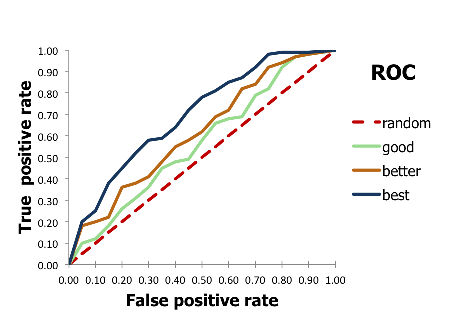
\includegraphics[width=0.8\linewidth]{images/roc.png}
		\caption{Example of ROC curve, source \cite{roc-curve}}
		\label{roc-curve}
	\end{center}
\end{figure}
\subsubsection{Evaluation of multiclass classificators}


http://stats.stackexchange.com/questions/2151/how-to-plot-roc-curves-in-multiclass-classification


http://stats.stackexchange.com/questions/44261/how-to-determine-the-quality-of-a-multiclass-classifier
\section{Parallel processing and scalability}
\section{Existing solutions}
	\subsection{Data mining}
	\textbf{Business}
		
	\textbf{Science}
	
	\textbf{Medicine}
	
	\textbf{Spatial}
	
		
	
	
	Other use cases cover such aspects as filtering unsolicited bulk e-mail \cite{naive-bayesian}. 
	\subsection{Machine learning}
		\subsubsection{Microsoft Azure Machine Learning}

\section{Conclusion}
This chapter reviewed a number of issues and concerns that might have risen through out the discussion about performing scalable text document classification. Different methods of classification and clusterization were discussed, including kNN and SVM.